\subsection{流域系统稳态转换的理论框架}

% 宋嘉熙 的 地理学报
本研究对流域系统人-水关系状态的分析植根于社会-生态系统的“稳态”概念,属于生态系统与社会-生态系统研究中,以弹性(Resilience,也被译为韧性)为核心的一组相关概念集合,通常使用“球-杯模型”或“折叠二分模型”进行描述(图\ref{ch2:fig:regime_shift})。
弹性是处于动态平稳的社会-生态系统面对变化时通过缓冲、适应或转变等方式响应以维持人类福祉的能力[30],稳态转换则是系统因大规模结构重组而在不同稳态之间发生迁移的现象。
以球-杯模型为例,不同稳态就像系统状态空间中凹陷的“杯子”,将系统实际状态则如同在不同凹陷间滚动的“小球”,状态空间的变化(参数驱动)或小球受到外力(外力驱动)时稳态转换都可能发生,致使系统状态在不同稳态间发生转换[8,36]。
变量驱动指的是当系统在外界条件变化不大时,直接参与系统反馈循环的核心变量不断积累变化或受到干扰所触发的稳态转换,作为替代进入已有的另一个稳态 (图\ref{ch2:fig:regime_shift}~B)。
参量驱动则是当外界条件(环境参数)发生变化时系统被诱发的稳态转换,新环境条件下系统的原先状态和替代稳态可能发生改变[7,8](图\ref{ch2:fig:regime_shift}~C)。
每次稳态转换的驱动模式会根据特定社会-生态系统而有所不同,但Rocha等人发现,无论以变量还是参量的形式出现,对于包括流域人-水系统在内的许多社会-生态系统,不断累积的人为干扰压力和气候变化都是最常见、最重要的两类稳态转换驱动因素[60,61]。
这两种驱动因素在较长的时间尺度下持续变化,致使系统稳态的“小球”突破临界点,触发人水关系的变化。

% Description of system regime shift by ball-cup model and fold bifurcation
\begin{figure}[htb] % use float package if you want it here
    \centering
    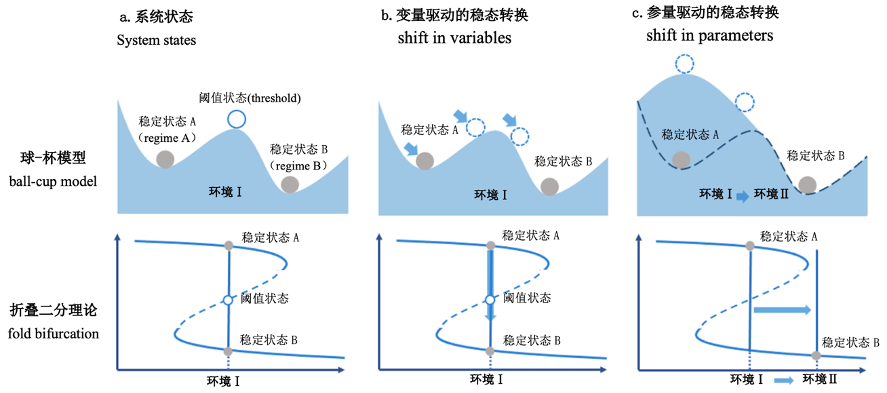
\includegraphics[width=\textwidth]{img/ch2/ch2_regime_shift.png}
    \caption[球-杯模型和折叠分岔理论对系统稳态转换的描述]{球-杯模型和折叠分岔理论对系统稳态转换的描述。
    假设系统中最多可能有2个稳定平衡状态,即稳定状态A(regime A)和稳定状态B(regime B)和1个阈值状态(threshold):
    a)环境Ⅰ条件下,球-杯模型(ball-cup model)和折叠二分理论(fold bifurcation)对系统各种状态的表征。
    b)系统稳态转换过程。变量驱动的稳态转换(shift in variables):环境Ⅰ不变时,处于稳定状态A的系统在干扰下自身突破阈值状态转换为稳定状态B。
    c)参量驱动的稳态转换(shift in parameters)。环境Ⅰ变为Ⅱ,迫使处于稳定平衡状态A的系统向新环境下仅存的稳定平衡状态B转换。(改自文献[7],[8])}\label{ch2:fig:regime_shift}
\end{figure}

% 地理学报
流域社会-生态系统的另一类常见人为干扰是水治理措施,但它不同于持续增加的人为压力,单独某个治理举措为稳态“小球”所施加的力也许是过小或过大的,且力的作用方向常常是不确定的,对于这类驱动力何时触发稳态转换需要“稳态循环”加以理解。
在每个稳态内的不同尺度下,社会-生态系统会自发历经开发(Growth)、保护(Senescence)、释放(Collapse)、更新(Renewal)四阶段的适应性循环[63],也有学者根据该循环将社会-生态系统框架下的治理总结为涌现(Emergence)、制度化(Institution)、更新(Renewal)三阶段(Chaffin and Gunderson, 2016)。
由于建立适应性治理体系是希望社会-生态系统状态维持在社会所需范围内,因此会产生“主动改变不良的社会-生态系统状态”与“调节并维持良好的社会-生态系统状态”两种不同的需要,通常这也是治理系统运作的主要思路。
转型治理关注社会-生态系统社会-生态系统的释放和更新阶段,强调适应性治理的实现,以及主动促使社会-生态系统完成状态的更新[64];协作治理则强调适应性治理制度化过程,旨在通过利益相关者间自组织的协作模式来实现社会-生态系统的开发与保护[65]。
转型治理企图通过自上而下的政策干预,积极将多尺度社会-生态系统转向所期待的状态[64];而协作治理的实现则常通过自下而上的手段,强调协作网络与协商制度的设计,从而建立具适应性的协作机制[68-70]。
无论自上而下或自下而上,治理流域系统产生的驱动力都既可能成为维持稳态的原因,也可能成为稳态转换的触发因素,需在分析其机制时应加以甄别。

\begin{figure}[htb] % use float package if you want it here
    \centering
    
\includegraphics{hello}
    \caption[社会-生态系统状态循环]{社会-生态系统状态循环与转型治理、协作治理的关系
    Fig.4  The relationship between social-ecological system adaptive cycle and transition / collaborative governance
    ①SES状态循环包括:开发阶段r,保护阶段K,释放阶段Ω,更新阶段α;图中展示旧的SES因转型治理而进入新的状态循环,并因协作治理的实现而延长开发保护阶段的过程;②转型治理可受其它尺度SES的影响[64,66];③协作治理的主要实现过程包括F-F-D(Face to Face Dialogue, 当面沟通),T-B(Trust-Building, 建立信任),C-P(Commitment to Process, 过程承诺),S-U(Shared Understanding, 信息对称),I-O(Intermediate Outcomes, 阶段成果)五步骤的循环[65,68,58]。}
    \label{fig:xfig0}
\end{figure}

\subsection{识别流域稳态与人水关系的变化}

% 宋嘉熙 的 地理学报
根据本研究对流域人水关系的定义,以及对稳态转换框架的认识,识别流域系统的稳态转换是分析人水关系变化过程的基础,分析其驱动力则是明晰变化机制的关键。
除了驱动因素外,系统稳态转换的发生可能致使系统现象(Phenomenal)、系统产出(Outcome)发生显著改变,或因级联效应触发其它的稳态转换(Cascading effect)。
既有经验研究中一些识别变化特征的常见方法包括:辨识系统互馈变量的趋势突变、识别其它解释变量变化轨迹的不连续性、检测系统结构-功能指标的变化信号等。
本章研究将驱动力(Drivers)、现象(Outcome)、与效应(Effects)认为是稳态转换的三核心要素,提出识别稳态转换应从其中多个要素的复合状态切入,分析关键特征的变化。
换言之,本研究中识别流域稳态时,须使用特征变化的识别方法对稳态转换的驱动力和现象/效应都进行分析或检验,确定流域系统内既存在明显的突变现象,又存在相应的稳态转换驱动力。

% 宋嘉熙 的 地理学报
黄河流域长时间受人类活动强烈干扰[48],流域系统内变量关系复杂存在诸多子系统(如水沙子系统、社会经济子系统、社会-生态子系统等),素来是稳态转换研究的代表性区域。
因此本章以黄河流域符合上述定义的稳态变化的实证研究为典型案例,总结了稳态转换研究中三种常见的分析路径如图\ref{ch2:fig:identifying}所示。
最常见的稳态转换识别,是聚焦于稳态转换过程中所表征出的现象,寻找合适的指标与标准识别系统互馈变量的趋势突变或其它相关解释变量的不连续性,对直接相关的变量进行检测。
当分析缺乏完整的现象变量数据资料而驱动力明确的稳态转换现象时,从驱动因素的阈值效应入手建立指标和标准,也可有效分析稳态转换过程。

结合本章先前对“人水关系”进行的严格定义,本研究识别人水关系变化过程及其机制的总体思路是:识别主导流域“自然-社会”二元水循环稳态的关联要素及其稳态变化现象,结合稳态转换的驱动机制(气候变化或人类活动?自上而下或自下而上?)分析利益相关者的与水圈要素过程的联系状态如何变换、因何变化。

\begin{figure}[!htb] % use float package if you want it here
    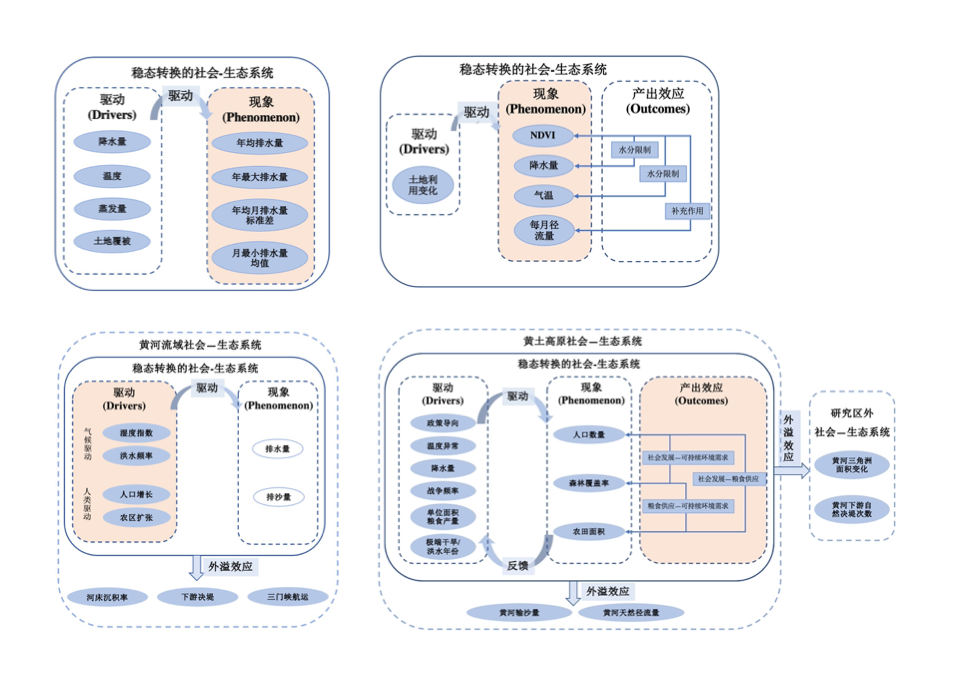
\includegraphics[width=\textwidth]{img/ch2/ch2_identifying.png}
    \caption[三种分析稳态转换的常见路径的实证研究案例]{三种分析稳态转换的常见路径的实证研究案例。
    蓝色背景椭圆框为可获取数据的变量,白色背景椭圆形框为不可获取数据的变量;双箭头线连接了两个变量,箭头线上蓝色背景方框表示产出效应的具体意义;粉色背景矩形框为判断系统多稳态和稳态转换过程的依据,即通过关键现象(a和b)、驱动因素的阈值效应(c)、系统效应的改变(d)识别并分析稳态转换;实线框为稳态转换的社会-生态系统边界。
    图中展示了四个典型研究:
    a)通过关键现象识别稳态转换后探寻驱动因素(改自文献[49]);
    b)通过关键现象识别稳态转换后分析系统产出效应 (改自文献[83],备注:该案例中驱动因素仅仅作用于NDVI而非全部现象变量);
    c)通过驱动因素的阈值识别稳态转换过程,并结合外溢效应验证(改自文献[48])。
    d)通过产出关系改变识别稳态转换过程,进一步分析驱动和外溢效应变化 (改自文献[65])。}\label{ch2:fig:identifying}
\end{figure}
